%!TEX root = ../../thesis.tex


\subsection{Earth's atmosphere, in the NIR}
\todo{move out of intro}
While the Earth's atmosphere is important life on Earth, it can be a nuisance for ground-based observations astronomical observations. While the atmosphere is mostly transparent in the visible, with only minor transmission and emission features, it is not uniformly transparent in the infrared. 

As light form astronomical sources passes through Earth's atmosphere, the molecular species absorb specific wavelengths (corresponding to molecular rotational and vibrational energy levels) densely populating the \nir{} with absorption lines, commonly referred to as telluric absorption. \Cref{fig:croppedmolecfitabsorbtion} contains the model telluric absorption spectrum for the atmosphere from 0.3--30\um{} at a high resolution of \textbf{XXXX} from~\citet{smette_molecfit_2015}. It clearly shows that there are regions where the atmosphere is mostly transparent (transmission of 1), with other wavelength regions (e.g. at 4.5\um) that are completely opaque.

\begin{figure}
    \centering
    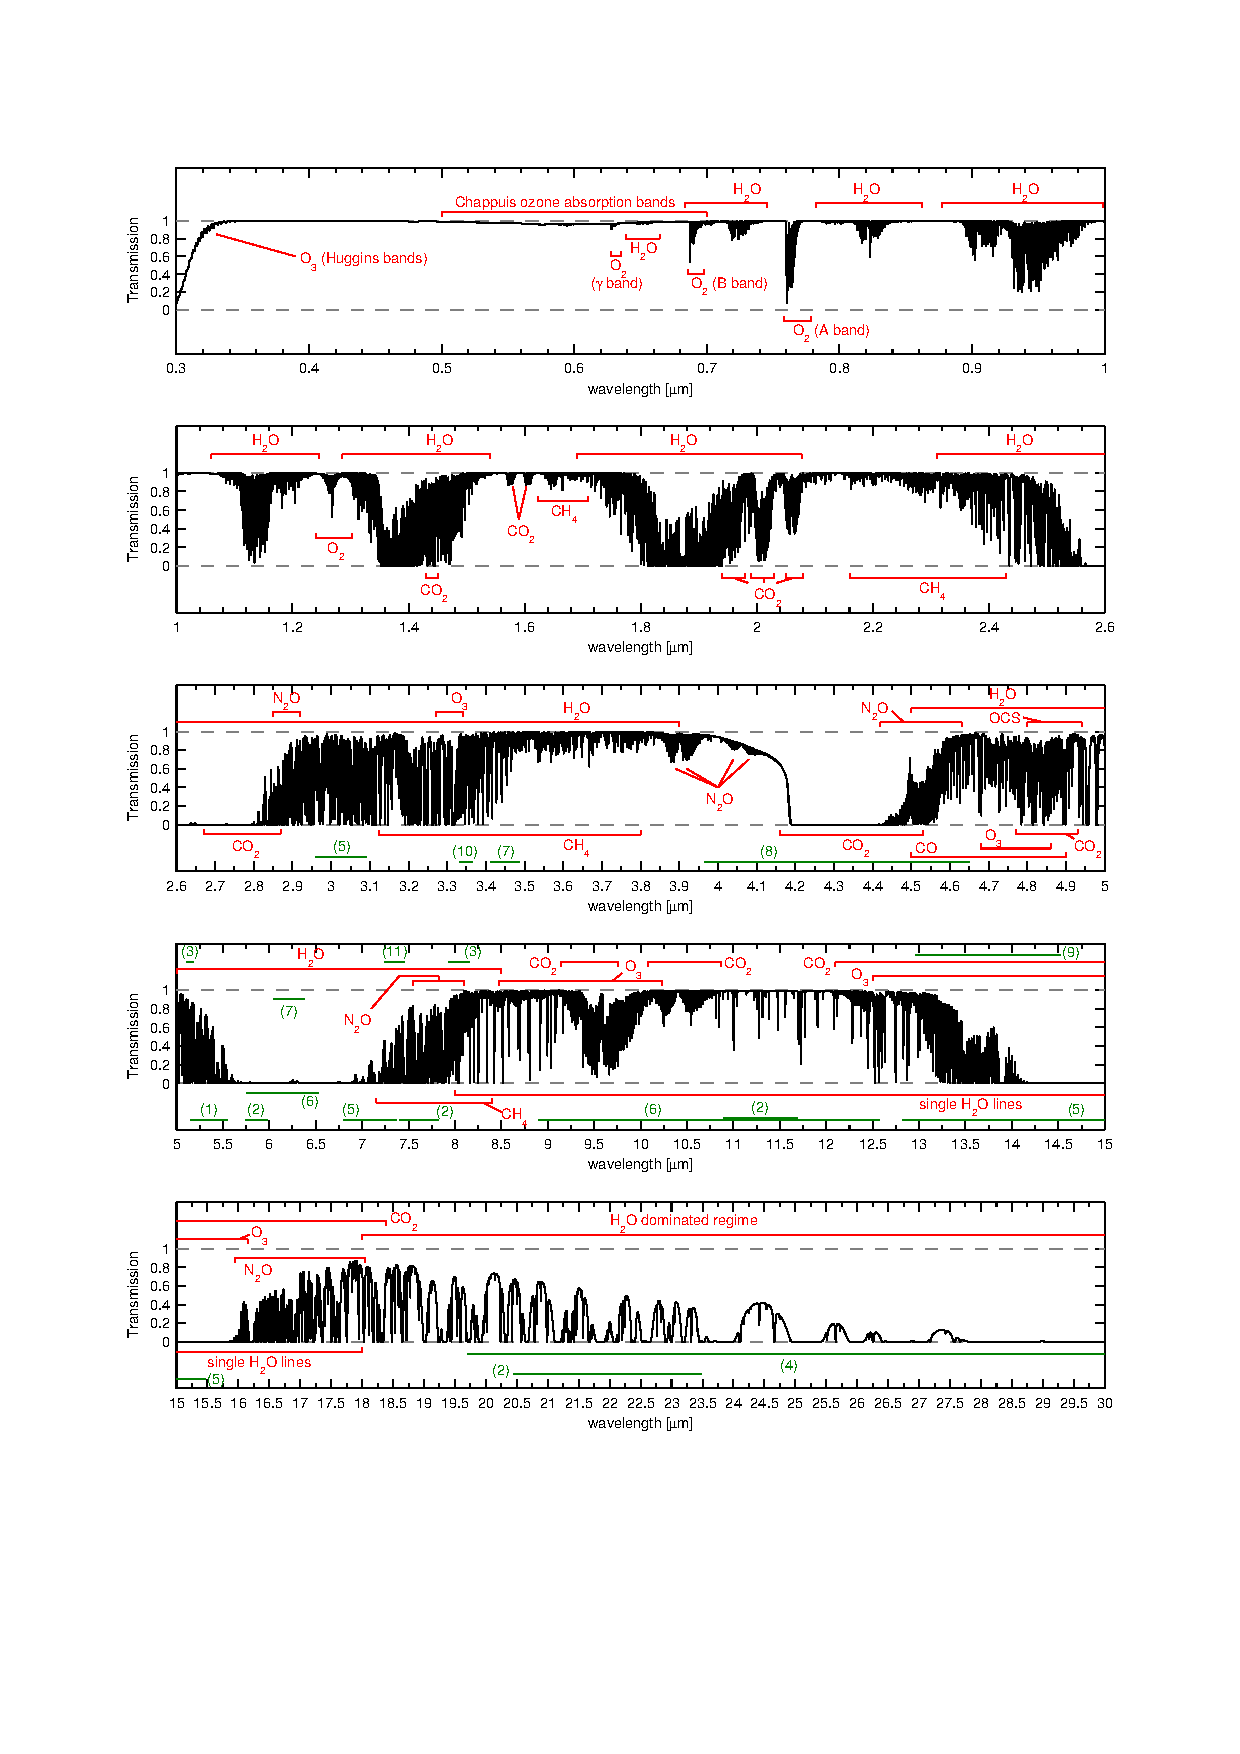
\includegraphics[width=0.9\linewidth]{figures/atmos_and_models/cropped_molecfit_absorption}
    \caption{Telluric absorption map from 0.3-30\um at a resolution of \textbf{XXXX}. ~\citet[][Figure~1]{smette_molecfit_2015}. The molecular species that are responsible for the large absorption features are indicated.
        Original caption:\textbf{add more here / see if original caption has anything else to add}}
    \label{fig:croppedmolecfitabsorbtion}
\end{figure}
\todo{Add original caption to~\cref{fig:croppedmolecfitabsorbtion}}

The windows of transmission defined the location of photometric bands in the infrared, with the common ones listed in \cref{tab:infrared_bands}~\citep[see e.g.][]{sterken_astronomical_1992, binney_galactic_1998}.
There are also variations on these bands for specific to different sites.
These photometric bands are chosen for high average photometric\footnote{Considering all photons in the band equally, regardless of wavelength (Very low resolution)} throughput, and do not consider the variable spectroscopic content inside the individual bands that becomes evident when observing at high resolution.

\begin{table}
    \caption{Standard infrared pass-bands.}
    \begin{tabular}{lcc}
        \toprule
        Band &  Central wavelength [\um] & Bandwidth [\um]\\
        \midrule
        Z & 0.9 & 0.06 \\
        Y & 1.05, 0.12 \\
        J & 1.25 & 0.38 \\
        H & 1.65 & 0.48 \\
        K & 2.2 & 0.4 \\
        L & 3.5 & 1.2 \\
        M & 4.8 & 0.6 \\
        N & 10.6 & 2.5 \\
        Q & 21 & 5.8 \\
        \bottomrule
    \end{tabular} \label{tab:infrared_bands} 
    e.g. \citep{binney_galactic_1998, sterken_astronomical_1992}   
\end{table}

The most prominent absorber in the infrared is water vapour (\si{H2O}) which is a strong absorber defining the photometric bands as seen in \cref{tab:infrared_bands}. Water vapour is mostly concentrated in the lower 5\,\si{\kilo\metre}, so infrared observatories are situated in dry places at high altitude. Even under ideal conditions the absorption of water vapour defines the IR bands. Other molecular species in the atmosphere are also important at various wavelengths, such as, \ce{CO}, \ce{CO2}, \ce{CH4}. 



When performing spectroscopy the spectrum of Earth's contaminates the spectrum of the intended target. In high-resolution spectroscopy the stellar and atmospheric lines can be resolved allowing for the identification and separation of the spectra. The removal or correction for the telluric lines is very important for accurate science, especially for detecting exoplanet atmospheres in which the species trying to be detected also reside in our atmosphere~\citep{snellen_orbital_2010, brogi_carbon_2014, dekok_detection_2013}.


\todo{telluric correction section now}

\textbf{ variability, and sensitivity to atmospheric conditions with modelling. }

Works such as \citet{snellen_orbital_2010}, fit and remove the telluric variation during a series of observations\footnote{51 spectrum of the same target in 180 minutes for \citet{snellen_orbital_2010}}, to remove telluric lines and detect the absorption lines of exoplanet atmospheres.


Other atmospheric species such as 


Telluric correction

Bailey 2007, Reiners ... smette 




The correction of observations from the contamination of Earth's atmosphere is a complex process.\textbf{
    The transmission is variable on many different time scales, the water vapour change is rapid, concentrations of atmospheric constituents, to seasonal and longer.}
Such as the increase in atmospheric \ce{CO2} causing anthropamorphic climate change this requires 6\% change to \ce{CO2} line depths since 2000 Molecfit paper?
There is also a variation with airmass, which depends on the observation angle in the sky and changes as targets move across the sky during the night. This is because the light will through a longer column of air.

other constituents, \ce{CO}, \ce{CO2}, \ce{CH4} \ldots{}, angle of observations.

An important consideration in detecting the constituents of planetary atmospheres is the characterization and removal of Earth's telluric lines.

e.g.\ 50\% error in \ce{CO2} detection on Mars atmosphere


Recently~\citet{ulmer-moll_telluric_2018} compared the telluric correction possible from three different synthetic telluric software against the standard star model.
Molecfit, a software from ESO was the most.

This is a growing field and there are other software available too, such as Telfit, ... and ..\ldots{}


Water vapour content has rapid variability.


\todo{finish this}


